\documentclass[11pt, dvipsnames, DIV=12]{scrreprt}
\usepackage{babel}

\usepackage[utf8]{inputenc}
\usepackage[T1]{fontenc}
\usepackage{natbib}
\bibliographystyle{abbrvnat}
\usepackage{subcaption}
\usepackage{booktabs}
\usepackage{multirow}
\usepackage{url}
\usepackage{tikz}
\usepackage{paralist}

\usepackage{ifthen}
\newcommand{\CC}[1][]{$\text{C\hspace{-.25ex}}^{_{_{_{++}}}}
\ifthenelse{\equal{#1}{}}{}{\text{\hspace{-.625ex}#1}}$}

\usepackage{bm}
\usepackage{amsmath}
\usepackage{amssymb}
\usepackage{amsthm}
\usepackage{amsfonts}
\usepackage{thmtools}		
\usepackage{mleftright}
\usepackage{stmaryrd}
\usepackage{nicefrac}
\usepackage{algorithm}
\usepackage{algorithmicx}
\usepackage[noend]{algpseudocode}
\renewcommand{\algorithmicrequire}{\textbf{Input:}}
\renewcommand{\algorithmicensure}{\textbf{Output:}}

% Fixes some spacing issues with braces.
\let\originalleft\left
\let\originalright\right
\renewcommand{\left}{\mathopen{}\mathclose\bgroup\originalleft}
\renewcommand{\right}{\aftergroup\egroup\originalright}

\theoremstyle{definition}
\newtheorem{theorem}{Theorem}
\newtheorem{conjecture}{Conjecture}
\newtheorem{proposition}[theorem]{Proposition}
\newtheorem{insight}{Insight}
\newtheorem{observation}{Observation}
\newtheorem{lemma}[theorem]{Lemma}
\newtheorem{corollary}[theorem]{Corollary}
\newtheorem{definition}[theorem]{Definition}
\newtheorem{example}[theorem]{Example}
\newtheorem{remark}[theorem]{Remark}
\newtheorem{claim}[theorem]{Claim}
\newtheorem{fact}[theorem]{Fact}
\usepackage{thm-restate}
\usepackage[mathic=true]{mathtools}
\usepackage{fixmath}
\usepackage{siunitx}

\usepackage{pifont}
\newcommand{\cmark}{\ding{51}}
\newcommand{\xmark}{\ding{55}}
\usepackage{blindtext}

\usepackage{todonotes}

\usepackage{enumitem}
\setlist[enumerate]{itemsep=0.2ex, topsep=0.5\topsep}
\setlist[description]{itemsep=0.2ex, topsep=0.5\topsep}
\setlist[itemize]{itemsep=0.2ex, topsep=0.5\topsep}


% Let cleveref and thmtools work together
\makeatletter
\def\thmt@refnamewithcomma #1#2#3,#4,#5\@nil{%
\@xa\def\csname\thmt@envname #1utorefname\endcsname{#3}%
\ifcsname #2refname\endcsname
\csname #2refname\expandafter\endcsname\expandafter{\thmt@envname}{#3}{#4}%
\fi
}
\makeatother


\usepackage[pagebackref,
pdfa,
hidelinks,
pdftex, 
pdfdisplaydoctitle,
pdfpagelabels,
pdfauthor={},
pdftitle={},
pdfsubject={},
pdfkeywords={},
pdfproducer={Latex with the hyperref package},
pdfcreator={pdflatex}
]{hyperref}

\usepackage[capitalise,noabbrev]{cleveref}   

\usepackage{microtype}
\usepackage{ellipsis}

\usepackage[scaled=0.86]{helvet}
\usepackage{lmodern}

% Bold. 
\newcommand{\mF}{\mathbf{F}}
\newcommand{\mG}{\mathbf{G}}
\newcommand{\mH}{\mathbf{H}}
\newcommand{\mL}{\mathbf{L}}
\newcommand{\mI}{\mathbf{I}}

\newcommand{\mW}{\mathbf{W}}
\newcommand{\ma}{\mathbf{a}}
\newcommand{\mb}{\mathbf{b}}
\newcommand{\mw}{\mathbf{w}}

\newcommand{\ba}{\ensuremath{{\bf a}}}
\newcommand{\bb}{\ensuremath{{\bf b}}}
\newcommand{\bc}{\ensuremath{{\bf c}}}

% Calligraphic.
\newcommand{\cC}{\mathcal{C}}
\newcommand{\cF}{\mathcal{F}}
\newcommand{\cG}{\mathcal{G}}
\newcommand{\cH}{\mathcal{H}}
\newcommand{\cN}{\mathcal{N}}
\newcommand{\cO}{\mathcal{O}}
\newcommand{\cP}{\mathcal{P}}
\newcommand{\cR}{\mathcal{R}}
\newcommand{\cS}{\mathcal{S}}
\newcommand{\cT}{\mathcal{T}}
\newcommand{\cU}{\mathcal{U}}
\newcommand{\cV}{\mathcal{V}}

% Sans serif.
\newcommand{\sC}{\mathsf{C}}

% Blackboard.
\newcommand{\Fb}{\mathbb{F}}
\newcommand{\Gb}{\mathbb{G}}
\newcommand{\Nb}{\mathbb{N}}
\newcommand{\Qb}{\mathbb{Q}}
\newcommand{\Rb}{\mathbb{R}}
\newcommand{\Zb}{\mathbb{Z}}

% Multiset Definition
\newcommand{\MSopen}{\{\!\!\{}
\newcommand{\MSclose}{\}\!\!\}}

% 1-WL+NN
\newcommand{\wlnn}{\text{1-WL+NN }}

\usetikzlibrary{calc}


\usepackage[auth-lg]{authblk}
\newcommand{\cm}[1]{{{\textcolor{purple}{\textbf{[CM:} {#1}\textbf{]}}}}}


\renewcommand*{\Affilfont}{\large\normalfont}
\renewcommand*{\Authfont}{\normalfont}

\recalctypearea
\setcounter{Maxaffil}{2}

\title{\emph{A Theoretical and Empirical Investigation into the Equivalence of GNNs and 1-WL+NN}\\
\vspace{20pt}\small{\normalfont From the faculty of Mathematics, Physics, and Computer Science for the purpose of obtaining the academic degree of Bachelor of Sciences.}
}
\author{Eric Tillmann Bill}
\affil{\vspace{100pt}}

\author{Supervision:\\Prof. Dr. rer. nat. Christopher Morris}
\affil{Informatik 6\\RWTH Aachen University}

\date{\vspace{-30pt}}

\renewcommand{\thesection}{\arabic{section}}

\begin{document}

\maketitle
\tableofcontents
\newpage



\section{Introduction}
Graphs are ubiquitous in various fields of life. Despite not always being explicitly identified as such, the graph data model's flexibility and simplicity make it an effective tool for modeling a diverse range of data. This includes unexpected instances, such as modeling text or images as a graph, as well as more complex instances like chemical molecules, citation networks, or connectivity encodings of the world wide web (\cite{Mor+2020,Sca+2009}).
Although machine learning has achieved remarkable success with images and text in the last decade, the lack of a significant breakthrough in machine learning for graphs can be attributed to the model's inherent flexibility and simplicity. While nodes in simple applications may be organized sequentially, as in text, or in a grid-like fashion, as in images, information in graphs can be arranged in more complex ways such as trees, acyclic graphs, or cyclic graphs. This complexity presents a significant challenge in developing a general machine-learning framework capable of accommodating all forms of graph inputs.


In recent years, there has been a significant amount of research conducted to investigate Graph Neural Networks (short GNNs). Among the most promising approaches are those utilizing the message-passing architecture, which was introduced by \cite{Gil+2017} and \cite{Sca+2009}. Empirically, this framework has demonstrated strong performance across various applications (\cite{Kip+2017, Ham+2017, Xu2018}). However, its expressiveness is limited, as has been proved by the works of \cite{Morris2018}, as well as \cite{Xu2018}. These works establish a connection to the commonly used Weisfeiler-Leman\footnote{Based on https://www.iti.zcu.cz/wl2018/pdf/leman.pdf, we will use the spelling ''Leman'' here, as requested by A. Leman, the co-inventor of the algorithm.} algorithm (short 1-WL), originally proposed by \cite{Wei+1968} as a simple heuristic for the graph isomorphism problem. In particular, it has been proven that a GNN based on the message-passing architecture can at most be as good as the 1-WL algorithm in distinguishing graphs. Furthermore, the 1-WL method demonstrates numerous similarities with the fundamental workings of the GNN architecture. It is therefore commonly believed that both methods are to some extent equivalent in their capacity.

In this work, we introduce a novel framework, which we coined ''1-WL+NN,'' which involves applying the 1-WL algorithm to an input graph, followed by further processing of the resulting information using a feed-forward neural network. Thereby, we obtain a trainable framework that is suited for all kinds of graph-related tasks, such as graph classification, node regression, and more.

In this thesis, we will conduct an extensive analysis of the newly proposed framework ''1-WL+NN'' and its connection to GNNs. The work will be divided into two main parts. Firstly, we will establish the equivalence of both frameworks in terms of their expressiveness. Specifically, we want to show that for every function computed by a GNN, there exists a suitable model based on the ''1-WL+NN'' framework with optimal parameters that compute the same function.

Secondly, we will undertake an empirical analysis of the performance of our proposed framework, by testing various configurations and comparing them to state-of-the-art GNN models, that are based on the message-passing architecture. Additionally, we will explain potential observable differences between the two frameworks, despite their shared similarities. Finally, the thesis will conclude with recommendations for further research based on these findings.

\section{Related Work}
\subsection{Graph Neural Networks}
In recent years, machine learning models have experienced a surge in popularity due to their significant performance advantages over conventional methods and their ability to autonomously adapt to their tasks. However, a closer examination of the applications where these models are been used reveals that they are highly specialized for the specific input of each application. For instance, modern convolutional neural networks (short CNNs) are designed to take in fixed-sized, grid-like data structures such as images, while modern language models process sequential data like textfiles.

The relevance of graphs to these examples lies in the fact that graphs can be used to model various types of inputs across many applications, and they provide a more general framework for modeling data. To illustrate, an image can be modeled as a graph for a CNN, where each pixel corresponds to a node in the graph holding the brightness value for each color value, and each node is connected to its neighboring pixels. Similarly, for sequential data like textfiles, one can encode a directed graph where each word in this file is represented as a node with the word as a feature, and it is connected outgoingly to the next following word. With these examples, we wanted to highlight the flexibility of how graphs can model data, however, this is also problematic, as this makes it particularly hard to construct a general machine-learning model on graphs. Levering any constraints on the format or size of the input can significantly limit the model's generality, and since graphs sizes and formats can vary within their applications, e.g. classification of molecules (\textsc{PubChem} \cite{Mor+2020}), the need for a general model is of great interest.

From the work of \cite{Gil+2017}, as well \cite{Sca+2009}, the so-called message-passing architecture emerged for Graph Neural Networks (short GNNs). This can be understood as a framework that never changes its input graph structurally and only modifies the node's features in each layer. In more detail, in each layer, a GNN based on the message-passing architecture, computes for each node a new feature, based on its current feature and the features of its neighbors. Later in section \ref{sec:GNN Defintion}, we will give a more formal definition of this architecture.
Throughout this thesis, I will use the term GNN and message-passing architecture interchangeably.


\subsection{Weisfeiler and Leman Algorithm}
The (1-dimensional) Weisfeiler-Leman algorithm (short 1-WL), proposed by \cite{Wei+1968}, was initially designed as a simple heuristic for the \textit{graph isomorphism problem}, but due to its interesting properties, its simplicity, and its good performance, the 1-WL algorithm gained a lot of attention from researchers across many fields. One of the most noticeable of these properties is, that the algorithm color codes the nodes of the input graph in such a way, that in each iteration, each color encodes a local learned substructure.

It works by coloring all nodes in each iteration the same color that fulfill two properties: 1. the nodes already share the same color and 2. the frequencies of the colors of their neighbors are equal. The algorithm continues as long as the number of colors changes in each iteration.
For determining whether two graphs are non-isomorphic, the heuristic applies the algorithm to both graphs simultaneously and concludes that the graphs are non-isomorphic as soon as the number of occurrences of a color is different between the graphs. We present a more formal definition of the algorithm later in the section \ref{sec:1-WL Definition}.

Since the \textit{graph isomorphism problem} is difficult to solve due to it being \textsf{NP}\textit{-complete}, the 1-WL algorithm, running in polynomial deterministic time, cannot solve the problem completely. Moreover, \cite{Cai1992} have constructed counterexamples of non-isomorphic graphs that the heuristic fails to distinguish, e.g. figure \ref{1-WL Counter Example}. However, following the work of \cite{Bab+1979}, this simple heuristic is still quite powerful and has a very low probability of failing to distinguish non-isomorphic graphs when both graphs are uniformly chosen at random.

To overcome the limited expressiveness of the 1-WL algorithm, it was generalized to the k-dimensional Weisfeiler-Leman algorithm (short $k$-WL), which works with $k$-tuples over the set of nodes. Interestingly, this created a hierarchy for the expressiveness of determining non-isomorphism, such that for all $k \in \mathbb{N}$ there exists a pair of non-isomorphic graphs that can be distinguished by the $(k+1)$-WL but not by the $k$-WL (\cite{Cai1992}).

\subsection{Connections between GNNs and the WL algorithm}\label{sec:conn gnn and 1wl}
A connection between GNNs based on the message-passing architecture and the 1-WL algorithm seems quite natural since both share similar properties in terms of how they process graph data. Most noticeably, both methods never change the graph structurally, since they only compute new node features in each iteration. And additionally, both methods use a 1-hop neighborhood aggregation as their basis for the computation of the new node feature. Following this intuition of both methods being very similar, many authors showed a theoretical connection between these methods. \cite{Morris2018}, as well as \cite{Xu2018}, showed that GNN's expressiveness power is upper bounded by the 1-WL in terms of distinguishing non-isomorphic graphs. In addition, \cite{Morris2018} also proposed a new $k$-GNN architecture that works over the set of subgraphs of size $k$. Interestingly, the authors showed that the proposed hierarchy over $k \in \mathbb{N}$ is equivalent to the $k$-WL hierarchy in terms of their expressive in distinguishing non-isomorphic graphs, meaning if there exists a $k$-GNN that can distinguish two non-isomorphic graphs than it is equivalent to say that the $k$-WL algorithm can distinguish these graphs as well.

\section{Preliminaries}
We first introduce a couple of notations that will be used in this thesis. With $[n]$, we denote the set $\{1, \ldots, n\} \subset \mathbb{N}$ for any $n \in \mathbb{N}$ and with $\MSopen \ldots \MSclose$ we denote a multiset which is formally defined as a 2 tuple $(X, m)$ with $X$ being a set of all unique elements and $m: X \rightarrow \mathbb{N}_{\geq 1}$ a mapping that maps every element in $X$ to its number of occurrences in the multiset.

\subsection{Graph Framework}
A graph is denoted by $G$ and is a 3 tuple $G:= (V, E, l)$ that consists of the set of all nodes $V$, the set of all edges $E \subseteq V \times V$ and a label function $l: M \rightarrow \Sigma$ with $M$ being either $V, V \cup E$ or $E$ and $\Sigma \subset \mathbb{N}_0$ a finite alphabet. Moreover, let $\mathcal{G}$ be the set of all finite graphs. Note, that our definition of the label function allows for graphs with labels either only on the nodes, only on the edges, or on both nodes and edges. Sometimes the values assigned by $l$ are called features, but this is usually only the case when $\Sigma$ is multidimensional, which we do not cover in this thesis. In addition, although we have defined it this way, the labeling function is optional, and in cases where no labeling function is given, we add the trivial labeling function $f_0: V(G) \rightarrow \{0\}$. Further, $G$ can be either directed or undirected, depending on the definition of $E$, where $E \subseteq \{(v,u) \mid v,u \in V\}$ defines a directed and $E \subseteq \{(v, u), (u,v) \mid v,u \in V, v\neq u\}$ defines an undirected graph. Additionally, we will use the notation $V(G)$ and $E(G)$ to denote the set of nodes of $G$ and the set of edges of $G$ respectively, as well as $l_G$ to denote the label function of $G$. With $\mathcal{N}(v)$ for $v \in V(G)$ we denote the set of neighbors of $v$ with $\mathcal{N}(v) := \{u \mid (u, v) \in E(G)\}$.

A coloring of a Graph $G$ is a function $C: V(G) \rightarrow \mathbb{N}_0$ that assigns each node in the graph a color (here a positive integer). Further, a coloring $C$ induces a partition $P$ on the set of nodes, for which we define $C^{-1}$ being the function that maps each color $c \in \mathbb{N}_0$ to its class of nodes with $C^{-1}(c) = \{ v\in V(G) \mid C(v) = c\}$. In addition, we let $h_{G, C} = \MSopen C(v) \mid v \in V(G) \MSclose$ be the histogram of graph $G$ with coloring $C$, that contains for every color in the image of $V(G)$ under $C$ the color and its frequency.

\subsection{Permutation-invariance and -equivariance}
We use $S_n$ to denote the symmetric group over the elements $[n]$ for any $n > 0$. $S_n$ consists of all permutations over these elements. Let G be a graph with $V(G) = [n]$, applying a permutation $\pi \in S_n$ on G, is defined as $G_\pi := \pi \cdot G$ where $V(G_\pi) = \{\pi(1), \ldots, \pi(n) \}$ and $E(G_\pi) = \{ (\pi(v), \pi(u)) \mid (v,u) \in E(G)\}$. We will now introduce two key concepts for classifying functions on graphs. Let $f: \mathcal{G} \rightarrow \mathcal{X}$ be an arbitrary function and let $V(G) = [n]$ for some $n \in \mathbb{N}$:\\
\begin{enumerate}
    \item The function $f$ is \textit{permutation-invariant} if and only if for all $G \in \mathcal{G}$ where $n_G := \mid V(G) \mid$ and for every $\pi \in S_{n_G}$: $f(G) = f(\pi \cdot G)$.
    \item The function $f$ is \textit{permuation-equivariant} if and only if for all $G \in \mathcal{G}$ where $n_G := \mid V(G) \mid$ and for every $\pi \in S_{n_G}$: $f(G) = \pi^{-1} \cdot f(\pi \cdot G)$
\end{enumerate}


\subsection{Weisfeiler and Leman Algorithm}\label{sec:1-WL Definition}
The Weisfeiler-Leman algorithm consists of two main parts, first the coloring algorithm and second the graph isomorphism test. We will introduce them in this section in this order. 

\subsubsection{The Weisfeiler-Leman graph coloring algorithm}
Let $G = (V,E,l)$ be a graph, then in each iteration $i$, the 1-WL computes a node coloring $C_i: V(G) \rightarrow \mathbb{N}$, which depends on the coloring of the neighbors and the node itself. In iteration $i=0$, the initial coloring is $C_0 = l$ or if $l$ is non existing $C_0 = c$ for an arbitrary constant $c \in \mathbb{N}$. For $i > 0$, the algorithm assigns a color to $v \in V(G)$ as follows:
\begin{align*}
C_i (v) = \textsf{RELABEL}((C_{i-1}(v), \MSopen C_{i-1}(u) \mid u \in \mathcal{N}(v) \MSclose))
\end{align*}

\noindent Where $\textsf{RELABEL}$ injectively maps the above pair to a unique, previously not used, natural number. The algorithm terminates when the number of colors between two iterations does not change, meaning the algorithm terminates after iteration $i$ if the following condition is satisfied:
\begin{align}
\forall v,w \in V(G):  C_i(v) = C_i(w) \iff C_{i+1}(v) = C_{i+1}(w)
\end{align}
Upon terminating we define $C_{\infty}$:= $C_i$ as the stable coloring. The algorithm always terminates after $n_G:= |V(G)|$ iterations (\cite{Gro2017}). Moreover, based on the work of \cite{Pai+87} about efficient refinement strategies, \cite{Car+82} proved that the stable coloring $C_\infty$ can be computed in time $\mathcal{O}(| V(G) | + |E(G)| \cdot log | V(G) |)$. For an illustration of this coloring algorithm, see figure \ref{Encoding example}.

\subsubsection{The Weisfeiler-Leman Graph Isomorphism Test}
To determine if two graphs $G, H \in \mathcal{G}$ are non-isomorphic (short $G \ncong H)$, one applies the 1-WL coloring algorithm on both graphs ''in parallel'' and checks after each iteration if the occurrences of each color are equal, else the algorithm would terminate and conclude non-isomorphic. Formally, the algorithm concludes non-isomorphic in iteration $i$ if there exists a color $c$ such that: 
\begin{align}
    |\{ v \in V(G) \mid c = C_i(v)\} | \neq |\{ v \in V(H) \mid c = C_i(v)\} |
\end{align}

Note that this test is only sound and not complete for the problem of graph isomorphism. Counterexamples where the algorithm fails to distinguish non-isomorphic graphs can be easily constructed, see Figure \Ref{1-WL Counter Example} which was discovered and proven by \cite{Cai1992}.

\begin{figure}[H]
    \centering
    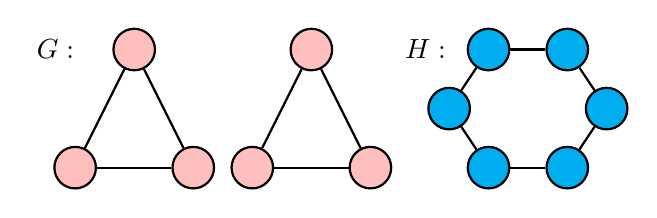
\begin{tikzpicture}

\tikzset{line/.style={draw,thick}}
\tikzset{arrow/.style={line,->,>=stealth}}
\tikzset{node/.style={circle,inner sep=0pt,minimum width=15pt}}

\draw (-1.0,0.75) node {$G:$};
\node[line,node,fill=pink] (x1) at (0, 0.75) {};
\node[line,node,fill=pink] (x2) at (-0.75, -0.75) {};
\node[line,node,fill=pink] (x3) at (0.75, -0.75) {};

\path[line] (x1) to (x2);
\path[line] (x1) to (x3);
\path[line] (x2) to (x3);

\node[line,node,fill=pink] (x1) at (2.25, 0.75) {};
\node[line,node,fill=pink] (x2) at (1.5, -0.75) {};
\node[line,node,fill=pink] (x3) at (3.0, -0.75) {};

\path[line] (x1) to (x2);
\path[line] (x1) to (x3);
\path[line] (x2) to (x3);

\draw (3.7, 0.75) node {$H:$};
\node[line,node,fill=cyan] (x1) at (3.75 + 0.25, 0) {};
\node[line,node,fill=cyan] (x2) at (4.25 + 0.25, 0.75) {};
\node[line,node,fill=cyan] (x3) at (5.25 + 0.25, 0.75) {};
\node[line,node,fill=cyan] (x4) at (5.75 + 0.25, 0) {};
\node[line,node,fill=cyan] (x5) at (5.25 + 0.25, -0.75) {};
\node[line,node,fill=cyan] (x6) at (4.25 + 0.25, -0.75) {};

\path[line] (x1) to (x2);
\path[line] (x2) to (x3);
\path[line] (x3) to (x4);
\path[line] (x4) to (x5);
\path[line] (x5) to (x6);
\path[line] (x6) to (x1);

\end{tikzpicture}
    \caption{An example of two graphs $G$ and $H$ that are non-isomorphic but cannot be distinguished by the 1-WL}
    \label{1-WL Counter Example}
\end{figure}

\subsection{1-WL+NN Framework}\label{sec:1-WL+NN Definition}
Let $\mathcal{G}_{\leq n} \subset \mathcal{G}$ be the set of all labeled graphs $G$ with $n$ or less nodes. We define the class \wlnn of functions over $\mathcal{X} \subseteq \mathcal{G}_{\leq n}$ as all functions that are comprised of an encoding function $F: \mathcal{X} \rightarrow R^C$, followed by a multilayer perceptron that takes vectors over $R^C$ as input in. In particular, the encoding function $F$ maps the final coloring $C^i_\infty$ of $G$ computed by the 1-WL algorithm to a vector in $R^C$. Note that $R$ can be an arbitrary domain, and $C \in \Nb$ is a constant.

As an example of a class following this definition, we present the bounded \wlnn classes that use the \emph{counting-encoding} function and are parametrized by $n, k \in \Nb$:

For $n, k \in \mathbb{N}$, let $\mathcal{X} = \{ G \in \mathcal{G}_{\leq n} \mid \forall x \in V(G) \cup E(G): l_G(x) \leq k \}$ be the set of all graphs with $n$ nodes and their label functions being bounded by $k$. We define the \emph{counting-encoding} Function $F: \mathcal{X} \rightarrow \mathbb{N}^C$ as the function that maps a graph $G$ to a vector $v \in \mathbb{N}^C$ such that the $i$.th component of $v$ is equal to the occurrence of the color $i$ in the final coloring computed by the 1-WL algorithm when applied to $G$. More formally, for $G \in \mathcal{X}$ let $C^i_\infty$ be the final coloring upon the termination of the 1-WL algorithm on $G$ and $h_{G}$ the respective color histogram. Than $F$ maps $G$ to a vector $v \in \mathbb{N}^C$, such that for all $i \in [C]: v_i = h_{G}(i)$. Important to note that due to the boundedness of the size of graphs $n$ and its labels $k$, there exists a minimal upper-bound $C$ for codomain $R^C$.

The bounded \wlnn class that uses the \emph{counting-encoding} function and is parametrized by $n$ and $k$, are a collection of functions of the format $f:\mathcal{X} \rightarrow \mathcal{Y}, G \mapsto \text{MLP} \circ F(G)$, where $\mathcal{Y}$ is a task-specific output set (e.g. labels of a classification task) and MLP is an arbitrary multilayer perceptron that takes in as input, vectors over $\Nb^C$. We will refer to this collection from now on by $\mathcal{C}_{n,k}$.

To illustrate how this encoding function works and why we coined it \emph{counting-encoding}, we will quickly introduce an example graph $G$. In figure \ref{Encoding example}, we give a visual representation of $G$ and its stable coloring after applying the 1-WL algorithm to it. The \emph{counting-encoding} function $F$ counts through all colors $i \in [C]$ and sets each $i$.th component to the number of occurrences in the final coloring. Therefore the respective color histogram $h_G = \MSopen 2, 2, 3, 4 \MSclose$ of $G$ is being mapped to $v \in \mathbb{N}^C$ with $v = (0, 2, 1, 1,0,  \dots ,0)^T$.
\begin{figure}[H]
    \centering
    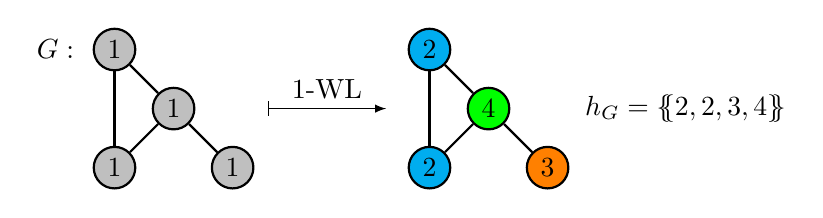
\begin{tikzpicture}
    \tikzset{line/.style={draw,thick}}
    \tikzset{arrow/.style={line,->,>=stealth}}
    \tikzset{node/.style={circle,inner sep=0pt,minimum width=15pt}}
    
    \draw (-1.5,0.75) node {$G:$};
    \node[line,node,fill=lightgray] (x1) at (-0.75, 0.75) {1};
    \node[line,node,fill=lightgray] (x2) at (-0.75, -0.75) {1};
    \node[line,node,fill=lightgray] (x3) at (0.75, -0.75) {1};
    \node[line,node,fill=lightgray] (x4) at (0, 0) {1};
    
    \path[line] (x1) to (x2);
    \path[line] (x1) to (x4);
    \path[line] (x2) to (x4);
    \path[line] (x3) to (x4);

    \draw [|-latex] (1.2,0) -- node [text width=2.5cm,midway,above,align=center ] {1-WL} (2.7,0);
    

    \node[line,node,fill=cyan] (x1) at (-0.75 + 4.0, 0.75) {2};
    \node[line,node,fill=cyan] (x2) at (-0.75 + 4.0, -0.75) {2};
    \node[line,node,fill=orange] (x3) at (0.75 + 4.0, -0.75) {3};
    \node[line,node,fill=green] (x4) at (0 + 4.0, 0) {4};
    
    \path[line] (x1) to (x2);
    \path[line] (x1) to (x4);
    \path[line] (x2) to (x4);
    \path[line] (x3) to (x4);

    \draw (6.5, 0.0) node {$h_G = \MSopen 2, 2, 3, 4 \MSclose$};

    
    
    \end{tikzpicture}

    \caption{An example of the final coloring computed by applying the 1-WL algorithm on the graph $G$. The graph $G$ consists of $4$ nodes with all their labels being initially $1$.}
    \label{Encoding example}
\end{figure}

\subsection{Graph Neural Networks (Message Passing)}\label{sec:GNN Defintion}
Let $G = (V, E, l)$ be an arbitrary graph. A Graph Neural Network (GNN) is a composition of multiple layers where each layer $t$ passes a vector representation of each node $v$ or edge $e$ through $f^{(t)}(v)$ or $f^{(t)}(e)$ respectively and retrieves thereby a new graph that is structurally identical but has new feature information. Note that in the following we will restrict the definition to only consider node features, however, one can easily extend it to also include edge features. 

To begin with, we need a function $f^{(0)}: V(G) \rightarrow \mathbb{R}^{1 \times d}$ that is consistent with $l$, that translates all labels into a vector representation. Further, for every $t > 0$, $f$ is of the format:
\begin{align}
f^{(t)}(v) = f^{W_{1,t}}_{merge} (f^{(t-1)}(v), \  f^{W_{2,t}}_{agg}( \MSopen f^{(t-1)}(w) \mid w \in \mathcal{N}(v) \MSclose ))
\end{align}

\noindent Where $f^{W_{1,t}}_{merge}$ and $f^{W_{2,t}}_{agg}$ are arbitrary differentiable functions with $W_{1,t}$ and $W_{2,t}$ their respective parameters. Additionally, $f^{W_{2,t}}_{agg}$ has to be permuation-invariant. To demonstrate what kind of functions are typically used, we provide the functions used by \cite{Ham+2017}:
\begin{align}
    f^{W_{1,t}}_{merge}(v, agg) = \sigma (W^t \times \textsf{concat}(v, agg))\\
    f^{W_{2,t}}_{agg} = \max(\{ \sigma(W_{pool}^t \times f^{(t-1)}(u) + b \mid u \in \mathcal{N}(v))\})
\end{align}
\noindent Where $\sigma$ is a non-linear elementwise activation function; $W^k, W_{pool}$ and $b$ are trainable parameters and \textsf{concat} the concatenation function.

Depending on the objective, whether the GNN is tasked with a graph or only a node or edge task, the last layer differs. In the case of graph tasks, we add a permutation-invariant aggregation function to the end, here called $\textsf{READOUT}$, that aggregates over every node and computes a fixed-size output vector for the entire graph, e.g. a label for graph classification. In order to ensure that we can train the GNN in an end-to-end fashion, we require $\textsf{READOUT}$ to be also differentiable.

Let $\mathcal{A}$ be an instance of the described GNN framework. Further, let $K \in \mathbb{N}$ be the number of layers of the GNN, $\mathcal{G}$ the set of all graphs, $\mathcal{Y}$ the task-specific output set (e.g. labels of a classification task), then the overall function computed by $\mathcal{A}$ is:
\begin{align}
    &\mathcal{A}: \mathcal{G} \rightarrow \mathcal{Y}: x \mapsto f^{(K)} \circ \ldots \circ f^{(0)}(x)\\
    &\mathcal{A}: \mathcal{G} \rightarrow \mathcal{Y}: x \mapsto \textsf{READOUT} \circ f^{(K)} \circ \ldots \circ f^{(0)}(x)
\end{align}
As we require all aggregation functions to be permutation-invariant, the total composition $\mathcal{A}$ is permutation-invariant, and similarly, it is also differentiable. This enables us to train $\mathcal{A}$ like any other machine learning method in an end-to-end fashion, regardless of the underlying encoding used for graphs. This definition and use of notation are inspired by \cite{Morris2018} and \cite{Xu2018}.


\section{Main Part}
In this section, we will discuss the topic of this thesis. The thesis will be about the connection between graph neural networks based on the message-passing architecture and the 1-dimensional Weisfeiler-Leman algorithm. In particular, we will show a theoretical equivalence between GNNs and 1-WL+NN about their expressive in the first part. The second part will then be based on the results of the first part, an empirical analysis of the performance of GNNs and 1-WL+NN in different configurations. We will now introduce each part individually.

\subsection{Part I: Theoretical Proof of the Equivalence}
In this part, we will start by introducing the framework we coined 1-WL+NN, and demonstrate how a model of this framework can be used and trained in an end-to-end fashion for graph tasks. More importantly, we will build a connection to GNNs by trying to prove the following hypothesis:

\begin{quote}
\textit{
    For every function $\mathcal{A}$ computed by a GNN (definition in section \ref{sec:GNN Defintion}), there exists a 1-WL+NN model (definition in section \ref{sec:1-WL+NN Definition}) computing $\mathcal{A}$ as well.
}
\end{quote}
After proving this hypothesis formally, we can conclude that GNNs and 1-WL+NN models share the same capacity.

As of today, no known research to us investigates the relationship between these two frameworks. Nonetheless, several works, as outlined in \ref{sec:conn gnn and 1wl}, offer results that hint that this hypothesis may be valid.  Additionally, in the research conducted by \cite{Zopf2022}, the author empirically demonstrated how well the 1-WL test is in distinguishing non-isomorphic graphs across various datasets and used these results to give an upper bound on the actual classification task of the datasets when training an individual GNN on each dataset. This demonstrates, how the expressiveness of a graph algorithm on an arbitrary task is somehow limited by its capacity in distinguishing non-isomorphism.

Our approach for showing the validness of the hypothesis is, that the proving direction of ''1-WL+NN $\subseteq$ GNN'' is relatively trivial, as we can easily encode the 1-WL coloring algorithm in each GNN layer. The other direction, however, showing ''GNN $\subseteq$ 1-WL+NN'', is more challenging, for which we want to take inspiration from the proof presented in section 3.3 by \cite{Xu2018}. In more detail, we will try to prove that for every $n \in \Nb$ and arbitrary $k$, the class $\mathcal{C}_{n,k}$ (bounded class of \wlnn using the \emph{counting-encoding} function) is GNN-approximating. For this, we have to prove that there exists no other encoding function that is more expressive than the \emph{counting-encoding} function and we have to define what GNN-approximating means.

\subsection{Part II: Empirical Analysis and Comparison}
In this part, we will provide a comprehensive analysis of the performance of the 1-WL+NN framework by testing it on well-established benchmark datasets for GNNs. With this analysis we will try to answer the following questions:
\begin{enumerate}[label=Q\arabic*)]
    \item Which encoding of the feature space for 1-WL+NN framework has the best performance in generalizing? Does this result align with the results of research in other fields?
    \item Is there a performance difference between both frameworks, 1-WL+NN and GNNs, in generalizing? And if so, which one generalizes better after fewer training iterations? Is there an explanation for this behavior?
    \item Is one of the tasks better suited for a specific task setting? For example, is more suitable for graph classification? Why could this be, what is the fundamental difference between both frameworks leading to this result?
\end{enumerate}

As for the encoding functions and configuration, we want to test, we have not yet determined, which one to use. As this decision strongly depends on the results of part I, we can not specify current configurations for the \wlnn. As a baseline, we will use three well-tested and state-of-the-art GNNs:
\begin{enumerate}
    \item Graph Convolutional Network (short GCN) by \cite{Kip+2017} with and without training
    \item GraphSAGE developed by \cite{Ham+2017} with and without training
    \item Graph Isomorphism Network (short GIN) developed by \cite{Xu2018} with and without training
\end{enumerate}

For running the test cases, we will implement the 1-WL+NN with all its different configurations in Python using the open source library \textsc{PyTorch}\footnote{Open source machine learning framework that was originally developed by Meta AI and does now belong to the Linux Foundation umbrella. \href{https://pytorch.org}{https://pytorch.org}} and the open source extension \textsc{PyTorch Geometric}\footnote{Open source library that acts as an extension to PyTorch and allows for easy writing and training of graph neural networks. \href{https://pytorch-geometric.readthedocs.io/en/latest}{https://pytorch-geometric.readthedocs.io}}.

We will select the datasets to be used for benchmarking from the \textsc{TU-Dataset}, a curated collection of graph datasets that are highly suitable for training graph-based algorithms. This collection offers data from diverse applications of varying sizes, enabling us to thoroughly evaluate the performance of our frameworks on a wide range of inputs. This dataset is the result of extensive work by \cite{Mor+2020}.

\setcitestyle{numbers}
\bibliography{references}
\end{document}